\documentclass[mscthesis]{usiinfthesis}
\usepackage{lipsum}

\usepackage[linesnumbered,nosemicolon,noline]{algorithm2e}
\usepackage{algpseudocode}
\usepackage{environ}

%For substeps in algo environment
\newcounter{parentAlgoLine}
\SetKwBlock{BEGIN}{}{}

\makeatletter
\NewEnviron{substeps}{%
  \refstepcounter{AlgoLine}% <---- remove if necessary
  \protected@edef\theparentequation{\theequation}%
  \setcounter{parentAlgoLine}{\value{AlgoLine}}%
  \setcounter{AlgoLine}{0}%
  \def\theAlgoLine{\theparentAlgoLine.\arabic{AlgoLine}}%
  \BEGIN{\BODY}%
  \setcounter{AlgoLine}{\value{parentAlgoLine}}%
  \ignorespacesafterend
}
\makeatother

%For algo sub-state

\newcounter{algsubstate}
\renewcommand{\thealgsubstate}{\alph{algsubstate}}
\newenvironment{algsubstates}
  {\setcounter{algsubstate}{0}%
   \renewcommand{\State}{%
     \stepcounter{algsubstate}%
     \Statex {\footnotesize\thealgsubstate:}\space}}
  {}

\usepackage{listings}
\graphicspath{ {./figures/} }

\lstdefinelanguage{algebra}
{morekeywords={import,sort,constructors,observers,transformers,axioms,if,
else,end},
sensitive=false,
morecomment=[l]{//s},
}

% Variables
\newcommand\numberevents{59256 }

% For equations float
\usepackage{float}
\usepackage{aliascnt}
\newaliascnt{eqfloat}{equation}
\newfloat{eqfloat}{h}{eqflts}
\floatname{eqfloat}{Equation}

\newcommand*{\ORGeqfloat}{}
\let\ORGeqfloat\eqfloat
\def\eqfloat{%
  \let\ORIGINALcaption\caption
  \def\caption{%
    \addtocounter{equation}{-1}%
    \ORIGINALcaption
  }%
  \ORGeqfloat
}


\title{Alien species modelling via relational event models} %compulsory
%\specialization{Dependable Distributed Systems}%optional
%\subtitle{Subtitle: Reinventing the World} %optional 
\author{Niccol\`o Zuppichini} %compulsory
\begin{committee}
\advisor{Prof.}{Ernst-Jan Camiel}{Wit} %compulsory
\coadvisor{}{Igor}{Artico}{} %optional
\end{committee}
\Day{15} %compulsory
\Month{June} %compulsory
\Year{2022} %compulsory, put only the year
\place{Lugano} %compulsory

\dedication{To my beloved} %optional
\openepigraph{Someone said \dots}{Someone} %optional

%\makeindex %optional, also comment out \theindex at the end

\begin{document}

\maketitle %generates the titlepage, this is FIXED

\frontmatter %generates the frontmatter, this is FIXED

\begin{abstract}
% Topic introduction
During the last centuries human research on the interaction of species substantially intensified. However, we know little to nothing about the underlying process that shape the behaviours of alien species invasion across regions, countries and ecosystems.

% What we do here
In this paper we present a custom relational event model to study the the invasion of alien species, which are that are abnormally found outside of their native land. We describe the invasion of species as a temporal unidirectional bipartite species-region graph. Under this framework, we present a relation event model to model the study of co-invasion of species. We then apply this model to a subset of the dataset of \numberevents events ranging from 1800 to nowadays. The aim of this paper is hence to study what group of species have the tendency to co-invade a region.

% What we got
Using years of first records of 55451 invasion of alien species from 17 taxonomic groups spanning from 1800 to 2020 we show how a custom relational event model can be used to model the dynamics of species invasion. Due to the high size of the dataset, we also present an high performance implementation in python of our model.

%TODO should I put reference in introduction?
%TODO should I tak briefly about previous research?
%TODO introduce briefly computational challenge and HPC

\end{abstract}

%\begin{acknowledgements}
%\lipsum 
%\end{acknowledgements}

%\tableofcontents 
%\listoffigures %optional
%\listoftables %optional

\mainmatter

\chapter{Introduction}
% 1. Motivation. Why invasive species are a problem?
% 2. Briefly introduce the dataset
% 3. Briefly introduce how I will study the dataset
% 4. Briefly introduce how I will study the dataset
% 5. TODO briefly report the results

The rate at which alien species invade countries have increased over the last century and it's becoming an issue. The economic impact of alien species in Europe is estimated to be close to 13 billion dollars annually (\citet{intro:rate}). The interest in the study of the dynamics of alien species has been increasing over the years for this reason. Unfortunately, due to the complexity of the problem, is hard to come up with real actions. Intuitively, the invasion rate of species differs belonging to different taxonomic groups, however, a comprehensive global invasion dynamics study of the last centuries subdivided by taxonomic groups is still lacking. The dynamics of invasive species are driven by a multitude of factors simultaneously. These factors can be complex involving exogenous, endogenous, sociological, ecological and socio-economic factors. (\citet{intro:factors}). Given the complexity of the subject, it's important to develop a framework capable of studying and analyzing all the underlying effects simultaneously. 

Relational event modelling was first developed in the field of social network analysis (\citet{rem:butts}). A relational event is an interaction between a sender and a receiver at a specific timestamp. A relational event model studies the temporal sequence of such relational events. This framework has many advantages in the fact that it's able to study underlying temporal patterns, can efficiently deal with time-varying variables and it's a extremely adaptable hypothesis testing tool. Due to its versatility, in the years it's been applied in a large number of different fields such as animal-animal interaction (\citet{intro:cattle}), TODO cite 2 more.

%%TODO what did other people do?
%In the years, there have been a large number of different statistical approaches to relation event models to predict the appearance and spread of alien species.  
%
%%TODO review this
%To tackle the problem a dataset containing an extensive amount of invasive species in multiple geographic regions worldwide.  has been created (\citet{intro:dataset}). To further extend this study \citet{intro:ecological} fitted a REM on the dataset. \\
%%TODO I can't find the "Analysing ecological dynamics with relational event
%%models: the case of invasion events" paper


In this paper, we introduce a novel custom latent space relational event model to study the dynamics of co-invasion of species for a bipartite graph. The model takes into consideration multiple species simultaneously and studies the underlying relationship between different species co-invading regions by training on the most exhaustive source of first records of alien species in multiple regions in the world (TODO add ref). Traditional statistical tools, such as multidimensional scaling, fail to capture the similarity of nodes on this dataset due to its bipartite nature (i.e. no iteraction of the kind species-species and region-region). By studying the proximity of species and regions in the latent space, our model is capable of determining the group of species that have the tendency to co-invade a region and, in an analogous way, the group of regions that are more likely to be invaded by the same group of species. 

% Structure of the thesis
In chapter 2 we present an exaustive statistical background of the methods used for the reader. In chapter 3 we make a preliminary study of the  dataset of the alien species, provide a formulation of our latent space relational event model and propose an efficient algorithm to make inferences about the latent space. In chapter 4 we discuss implementation specifications and frameworks used. In chapter 5 we present our results by applying our model to the dataset. In chapter 5 we discuss our result.

\chapter{Background}

In this section we cover all the necessary background tools to develop our latent space relational event model. First, we introduce the concept of latent space. Then we cover in depth the relational event model framework. We introduce then the reader to the Kalmann Filter and the Expectation Maximization algorithms. 

\section{Latent space}
Given a relation event model with actors $V=(1...p)$ we define a vector space $V$ where each actor is a vector and the position of each vector is constrained by the distance to all the other vectors inside $V$. The distance in this space represents an affinity of each actor (i.e. vector) $i$ to create a connection to another actor $j$ in the relation event model. On the latent space the dynamics are assumed to be a random walk where the jumps between two time intervals are fixed


\begin{eqfloat}
\begin{equation}
    \begin{cases}
      x_k = x_{k-1} + \epsilon \; , \quad \epsilon ~ N(0, \Sigma) \\
      y_k \approx Poi(\lambda_k) \; , \quad \lambda^{s, r, k} = exp(\alpha-dist(x_s(k), x_r(k)) \cdot \lambda_1(k) \\
      \textrm{for} \; k = [0, ..., n]
    \end{cases}\,.
\label{eq:latent_randomwalk}
\end{equation}
\caption{Latent space}
\end{eqfloat}


\section{Relational event models (REM)}

Butts (\citet{rem:butts}) proposed a statistical modeling framework capable of analysing temporal information and evolution of a sequence of relational events. Given a set of receiver nodes, a set of sender nodes and a timeframe, a relational event \textit{e} is a triplet of a sender, a receiver and a timestamp. Depending on the underlying data, the sender set and receiver set may be disjoint to represent relationships. As instance, for studying the interaction between domestic animals the sender and receiver nodes belong to the same set (\citep{intro:cattle}). In contrast, when studying alien species invasion the species are the senders, the regions the receivers and they belong in disjoint sets. In general, a REM specifies time-varying event-rates for all dyads as a function of past events $E=(e_1, ..., e_N)$ where each event $e_i$ is defined as

\[
e_i = (s_i, r_i, t_i)
\]

In the above notation, $s_i \in S_{t_i} $ is the sender node, $r_i \in R_{t_i}$ the receiver node and $t_i$ is the time of the interaction. The sets $S_t, R_t$ respectively contain all the receiver and senders nodes at the current timestamp $t_i$. The cross product of these two sets is called \textit{risk set} $R_{t_i}$  \footnote{\label{riskset_footnote}To avoid confusion, note that Butts originally called this set the \textit{support set}.}



\[
R_{t_i} = S_{t_i} \times R_{t_i}
\]

The risk set is the set of all dyads for which an event $e_{t_i}$ may occurr, hence, at a given timestamp $t_i$ any relational event that occurs belongs to the risk set.

\[
R_{t_i} = \{e_{t_i} | e \; occurs \; at \; t_i\}
\]

The waiting time $T_{s,r}$ for a dyad to happend between a species $s$ and a region $r$ is exponentially distributed 

\[
T_{s,r} \approx Exp(\lambda(s, r, t)
\]


In the above equation, the hazard function $\lambda$ is defined as

\[
\lambda(s, r, t) = \lim_{\delta t \lim 0^+} \frac{P(t \leq T_{s,r} \leq t + \delta t | t \leq T_{s,r})}{\delta t}
\]

With some ease, the hazard function can be interpreted as the expected number of relational events in a time interval of lenght one, conditionally on the previous network events. The most common used hazard function is the Cox proportional hazard model. 

%%Theta is what thet called beta in Igor's paper (change it?)

\[
\lambda(s, r, t|G, \theta) = \lambda_0(t) \cdot \lambda_1(s, r, t|G, \theta)
\]
\[
\lambda_0(t) =  exp(dist(x_s, x_r))
\]
\[
\lambda_1(s, r, t|G, \theta) = exp(\sum_{j=1}^k \theta_j \cdot p_j(s, r|G)
\]

In this equation, $\lambda_0$ represents a baseline harzard for all dyads in the risk set exponentially distributed as the distance species-region in the latent space - the function $\lambda_1$ is the propability that an event at $t$ happens between a node $s$ and a node $r$. To estimate the parameters $\theta$ we maximise the partial likelihood of the Cox proportional hazard model 

%TODO this equation is wrong. lambda_0 does not cancel out. Check igor paper
\[
L(\lambda) =  \prod_{e \in E} \frac{\lambda_1(s_i, r_i, t_i | G, \theta}{ \sum_{s \in R_{t_i}} \lambda_1(s, r, t_i | G, \theta}
\]

Our research interest is twofold: to infer the structure of the latent space $X$ and to estimate the factors that increase, or decrease, the hazard function $\lambda$, more specifically, the parameter $\theta$.


\section{Extended Kalman Filter}

In 1960 R.E. Kalman published his paper describing a recursive solution to the discrete-data linear filtering problem (\citet{paper:kalmanfilter}). Since then, the Kalman filter gained extremely popularity in the machine learning and robotics resaerch field, particularly in area of autonomous navigation systems. The Kalman filter estimates the evolution of a process by using a feedback control. The filter first computes an estimation of the current proces state at some time, then, it tries to "filter out" the measurement  noise in a iterative process. As such, the Kalman filter equations can be subdivided into two categories: prediction step and update step. The prediction step is responsible for projecting forward in time the current state of the system. The update step takes the a-prior estimate given from the prediction step and by taking new measurements of the errror tries to obtain an improved a-posteriore estimate of the state. Indeed, the general form of the algorithm resembles a predictor-corrector algorithm for solving numerical problems. In this chapter I will provide a brief non-technical overview of the Kalman filter. A reader interested in a more in-depth discussion of the formulation of the Kalman filter is advised to read \citet{paper:Maybeck79}.

%A very “friendly” introduction to the
%general idea of the Kalman filter can be found in Chapter 1 of [Maybeck79], while a more complete
%introductory discussion can be found in [Sorenson70], which also contains some interesting
%historical narrative. More extensive references include [Gelb74], [Maybeck79], [Lewis86],
%[Brown92], and [Jacobs93].

\begin{figure}[h]
    \centering
    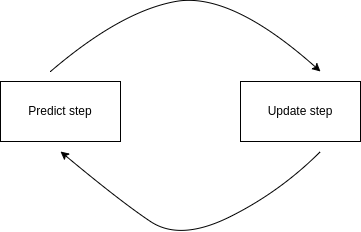
\includegraphics[width=0.25\textwidth]{kalman_diagram.png}
    \caption{The Kalman filter cycle. The time update forwards the current state estimate in time. The measurement update filters the noise out of the projected estimate.}
    \label{fig:kalman_cycle}
\end{figure}

Let's consider a non-linear system, $\epsilon$ captures uncertainity in the model, $v$ denotes the measurement noise. Both variables are white noises, random distributions with zero mean and uncorellated. 

\[
x_k \sim f(x_{k-1}) + \epsilon_k \; , \; \epsilon ~ N(0, \Sigma)
\]
\[
y_k \sim h(x_{k}) + v_{k} \; , \; v ~ N(0, \Delta)
\]

The initial state $x_0$ is a random vector with known mean and variance.

\begin{eqfloat}
\begin{equation}
\begin{array}{l}
\hat{x}_0 = \mu_0 = E[x_0] \\
\hat{V}_0 = V_0 = E[(x_0-\hat{x}_0)(x_0-\hat{x}_0)^T] 
\end{array}
\label{eq:kalman_init}
\end{equation}
\caption{Initialization}
\end{eqfloat}

%TODO see star1
Providing that $f, y \in C^1$, we can linearize the process around the mean. 


We define $\hat{x}_k^-$ to be our a-priori estimate of the state $x$ at time $k$, given the knowledge of the previous state. Similarly, we define $\hat{x}_k$ to be our a-posteriori estimate at time $k$ given a measurement $y_k$. The goal of the Kalman filter is to express the a-posteriori state $\hat{x}_k^-$ in terms of a linear combination of the a-priori state and the difference an actual measurement $y$ and a measurement prediction $H(\hat{x}_k^-)$ state. 

%\[
%\hat{x}_t \in span(\hat{x}_t^-, y_t - H\hat{x}_t^-) 
%\]
\[
\hat{x}_k = H\hat{x}_k^- + K (y_k - H_k \hat{x}_k^-)
\]
\[
V_k = (I-K_k H_k)V_k^-
\]


For a statistical motivation, I redirect the reader to \citet{paper:Maybeck79}. The difference $y_t - h_t(\hat{x}_t^-)$ is a residual of the estimation against the measurement, reflecting the error between the predicted measurement and the real measurement. The matrix $K$ is called Kalman gain matrix and is defined as 

\[
K_k = V_k^- H^T_k (H_k V_k^- H^T_k + R_k)^{-1}  \quad , \; H_k = \frac{d}{dx} h(x)
\]

The Kalman gain matrix goal is to minimise the a-posteriori covariance error matrix $V_t$ at time $t$. With some ease, a way of thinking $K$ is that as the measurement error covariance $R$ is close to zero the measurement $y$ is trusted more and the update is made with high precision. On contrary, if the a-priori estimate error covariance $P^-$ is close to zero, the acual measurement $y$ is less trusted and the predicted meausrement $H\hat{x}_t^-$ trust is increased. The "trust" is then reflected into the weights of the Kalman gain matrix $K$. We forecast an update of the estimation of $\hat{x} \approx x$

\begin{eqfloat}
\begin{equation}
\begin{array}{l}
\hat{x}_t^- = f(\hat{x}_{t-1}) \\
\hat{V}_t^- = J(x^f_{t-1}) V_{t-1} J(x^f_{t-1})^T + W_{t-1} Q_{t-1} W_{t-1}^T
\end{array}
\label{eq:kalman_predict}
\end{equation}
\caption{Prediction step}
\label{eq:kalmann_prediction}
\end{eqfloat}

Where $J(x)$ is the Jacobian of $f(x)$ and $Q_{t-1}$ the process noise covariance matrix.


\begin{eqfloat}
\begin{equation}
\begin{array}{l}
K_t = V_t^- H^T_t (H_t V_t^- H^T_t + R_t)^{-1} \\
\hat{x}_t = x_t^- + K (z_t - h(\hat{x}_t^-)) \\
V_t = (I-K_t H_t)V_t^-
\end{array}
\label{eq:kalman_update}
\end{equation}
\caption{Update step}
\label{eq:kalmann_update}
\end{eqfloat}

Where K is the Kalmann gain. By combining equations (\ref{eq:kalmann_prediction}), (\ref{eq:kalmann_update}) we get an algorithm for the Extended Kalmann Filter process is shown in Algorithm \ref{algo:kalmann}. 

\begin{algorithm}
\textbf{Initialize: }
\begin{substeps}
$\hat{x}_0 = \mu_0 = E[x_0]$ \;
$\hat{V}_0 = V_0 = E[(x_0-\hat{x}_0)(x_0-\hat{x}_0)^T]$  \;
\end{substeps}
\For{k=1,...,n}{
  Prediction step (Eq. \ref{eq:kalmann_prediction})
  \begin{substeps}
  $\hat{x}_t^- = f(\hat{x}_{t-1})$ \;
  $\hat{V}_t^- = J(x^f_{t-1}) V_{t-1} J(x^f_{t-1})^T + W_{t-1} Q_{t-1} W_{t-1}^T$\;
  \end{substeps}
  Update step (Eq. \ref{eq:kalmann_update})
  \begin{substeps}
  $K_t = V_t^- H^T_t (H_t V_t^- H^T_t + R_t)^{-1}$ \;
  $\hat{x}_t = x_t^- + K (z_t - h(\hat{x}_t^-))$\;
  $V_t = (I-K_t H_t)V_t^-$\;
  \end{substeps}
}
  \caption{Extended Kalmann Filter}
  \label{algo:kalmann}
\end{algorithm}

\section{Expectation Maximization}

A Maximum likelihood estimation seeks for a set of parameters that results in the best fit for the joint probability distribution of the data sample. However, a major limitation of this appraoch is that it assumes the dataset to be complete, which means that the dataset contains all the relevant variables. However, in most real world dataset this is generally not true. There may be variables that affect other variables but are hidden and not present in the dataset. These variables are referred to as latent variables (see section TODO add ref). Expectation maximization algorithm offes an appropiate forumlation of the maximum likelihood estimation taking into account latent variables in the optimization of model parameters. 

The expectation maximization algorithm is an iterative approach that cycles between two functions until convergence is reached. The procedure first estimates the values of the latent variables, then optimises the model. These two steps are repeated until convergence. This approach is extremely effective and is commonly used to estimate models with missing data such as clustering problems like Gaussian Mixture models. \\

%TODO I probably should move the whole algo to section 3 when we talk about our model
\begin{algorithm}
\While{not converged}{
  Expectation step
  \begin{substeps}
  Extended Kalmann filter \ref{eq:kalman_init} \;
  Smoother\;
  \end{substeps}
  Maximization step
}
  \caption{Model}
\end{algorithm}

\chapter{Materials and methods}

\section{Data}

%TODO add citation
The Alien Species First Records database (Seebens et al., 2017) contains the years of the first enstablishment of alien species in regions wordlwide. The original dataset has been later updated to include a more depth invasion dataset (TODO add papers where they update it) and the latest version includes (TODO put the numbers). 

We processed the dataset by taking the time interval from 1800 to 2020. By trimming the dataset, we removed 2495 relational event that happened before 1800. Specifically, we removed TODO species and TODO regions interactions. The subset of the dataset we take into consideration includes 19 taxonomic (listed in Tab. \ref{table:families}) families and 276 regions \footnote{Regions generally correspond to countries but there are also many islands large enough to be relevant.}. Considering all taxonomic families there's a total of 23039 species. As Fig. \ref{fig:hist_tax_fam} shows, most of the species in the dataset lie in the 'Vascular Platns" taxonomic family.

\begin{table}[H]
\centering
\begin{tabular}{|l|l|l|l|l|}
\hline
Algae      & Birds       & Fishes        & Mammals  & Vascular plants \\ \hline
Amphibians & Bryophytes  & Fungi         & Molluscs & Viruses         \\ \hline
Arthropods & Bryozoa     & Insects       & Reptiles &                 \\ \hline
Bacteria   & Crustaceans & Invertebrates & Spiders  &                 \\ \hline             
\end{tabular}
\caption{The 19 taxonomic families.}
\label{table:families}
\end{table}

\begin{figure}[H]
    \centering
    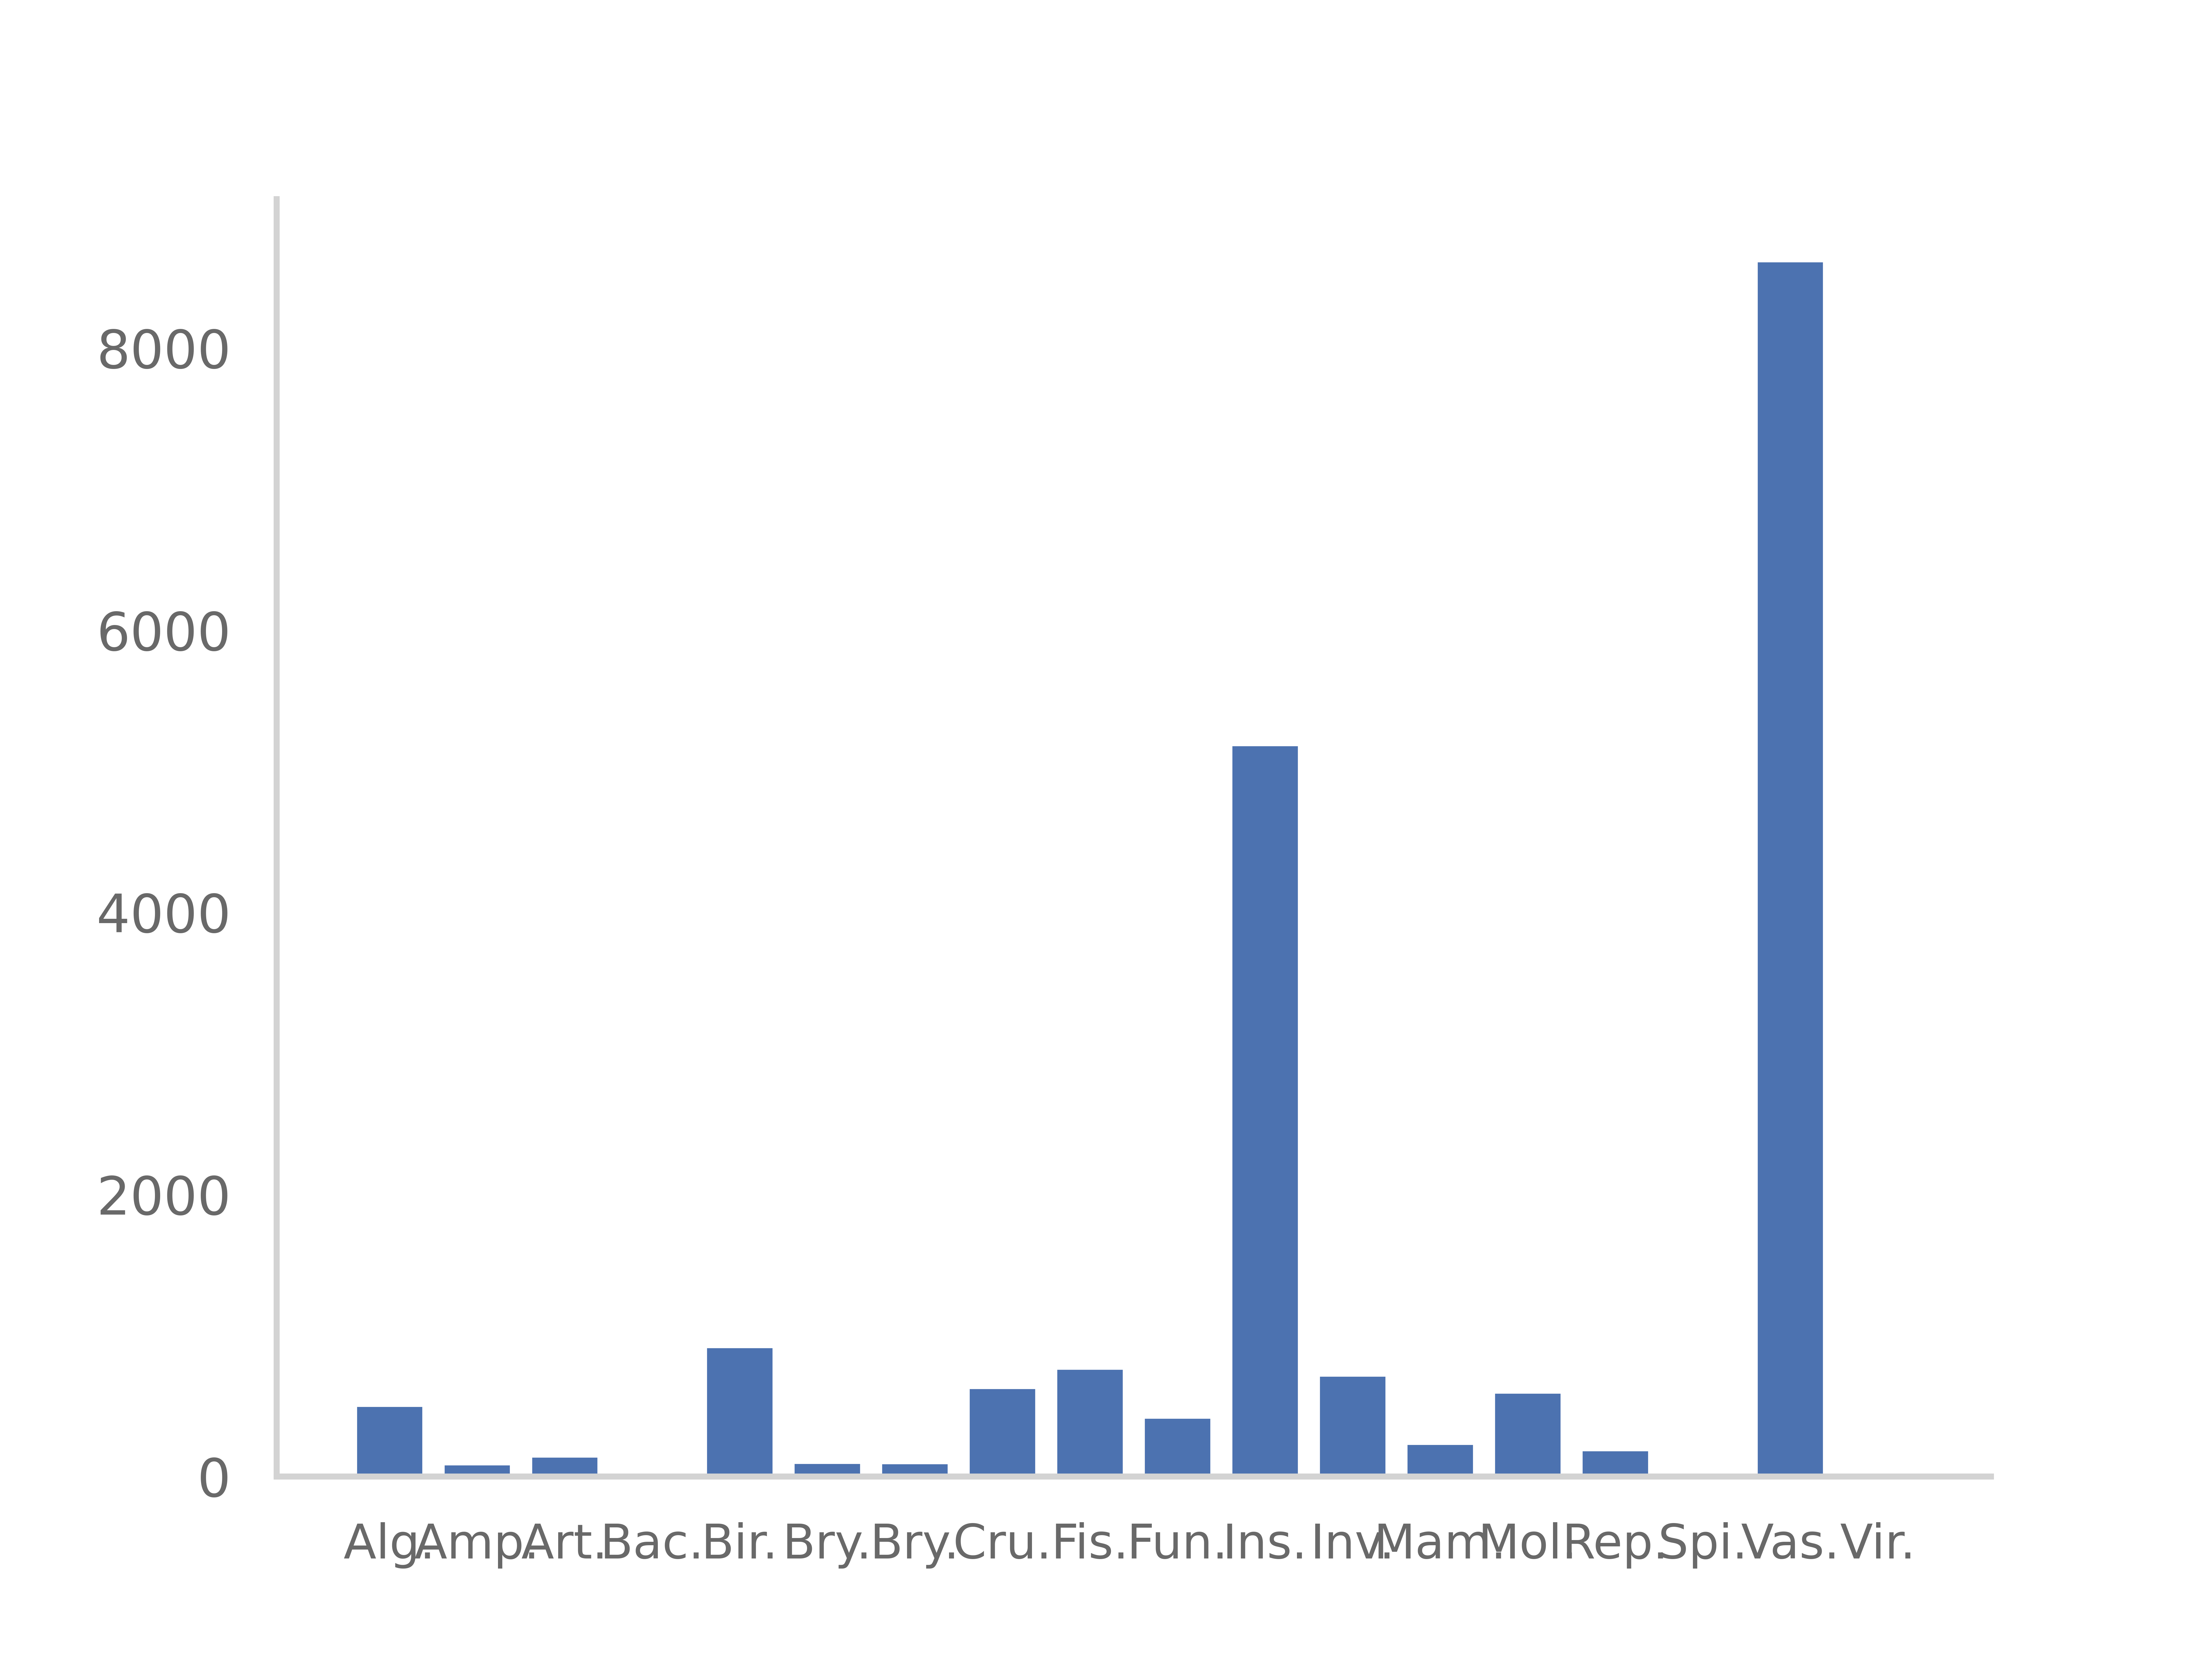
\includegraphics[width=0.75\textwidth]{histogram_taxfam}
    \caption{Histogram of Taxonomic Families and their respective number of species.}
    \label{fig:hist_tax_fam}
\end{figure}

%TODO Cite previous paper on ecological, they mentioned it
Intuitively due The amount invasion per year increases during time due to worldwide effects such as the grow of intercontinental trading etc...
\begin{figure}[H]
    \centering
    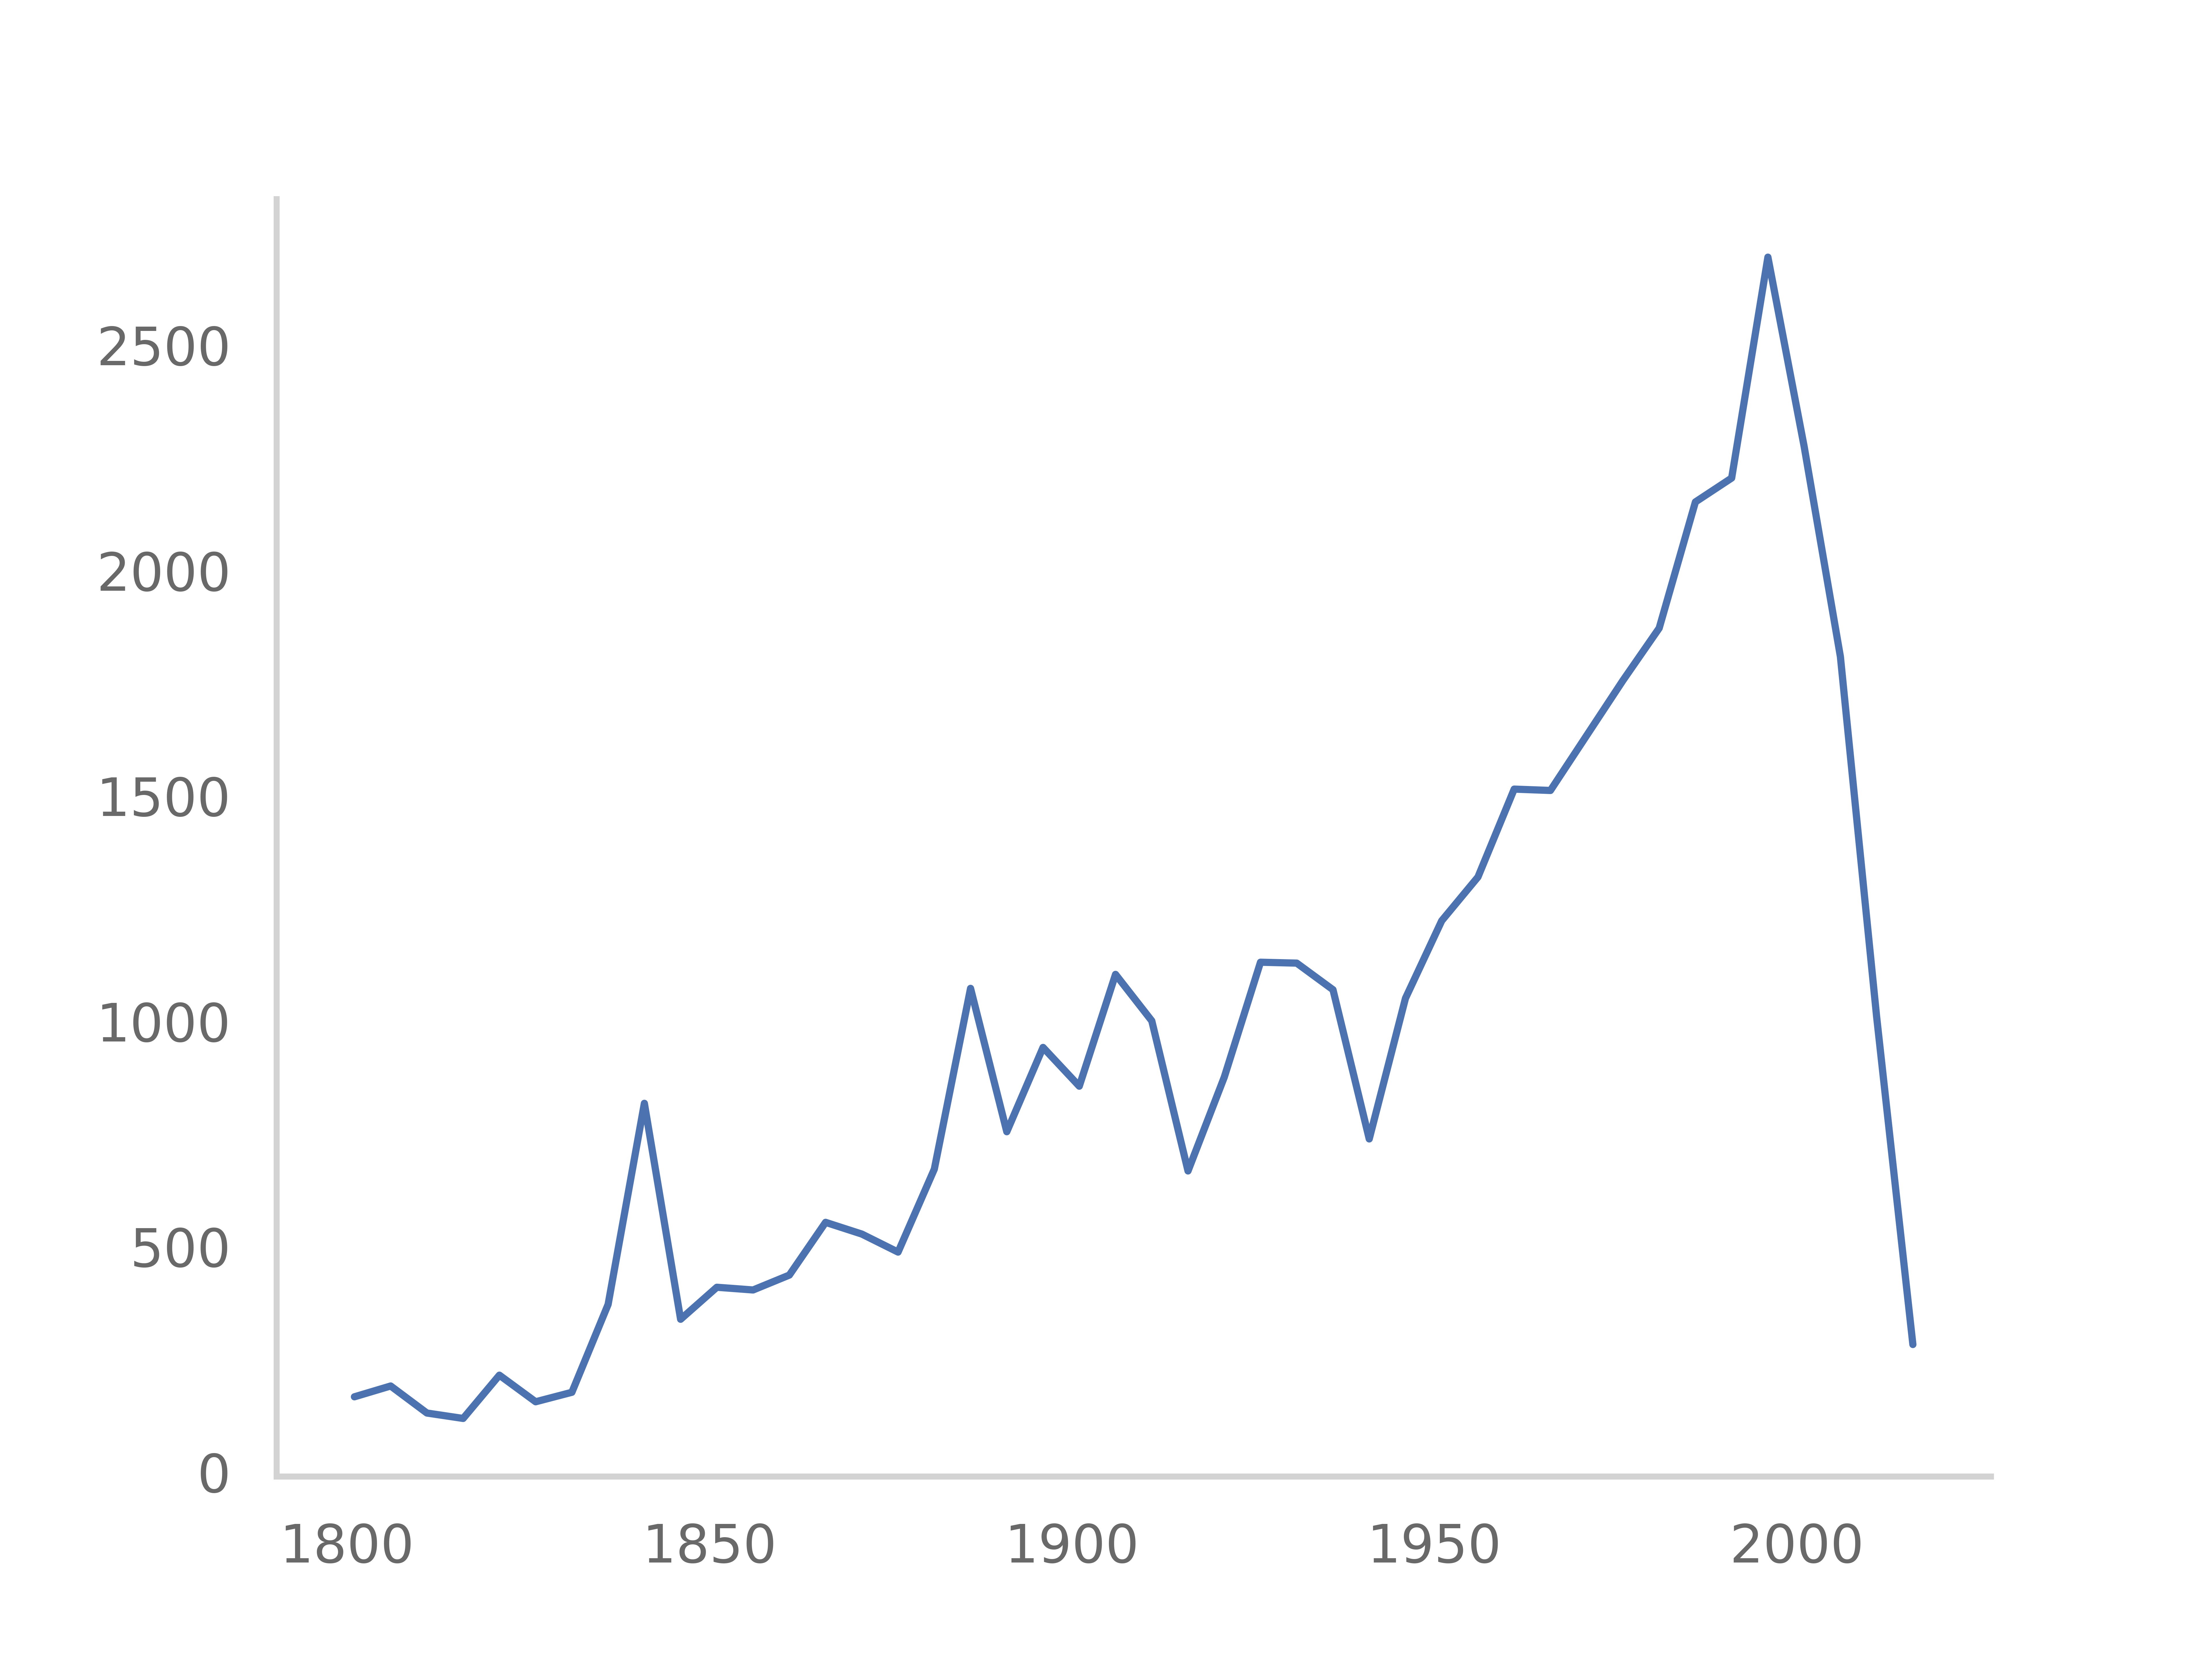
\includegraphics[width=0.75\textwidth]{invasion_per_year.png}
    \caption{Histogram of Taxonomic Families and their respective number of species.}
    \label{fig:pdf_invasion}
\end{figure}


The dataset is extremely sparse. Fig. \ref{fig:pdf_invasion} shows the probability density function of the number of region each species invades during the entire timeframe of the study (1800-2020).  The average number of invasion per species is 4. The distribution is largely skewed. The mean is 4, and standard deviation is 5. The are a few outsiders that invade

%TODO do the same plot for regions
\begin{figure}[H]
    \centering
    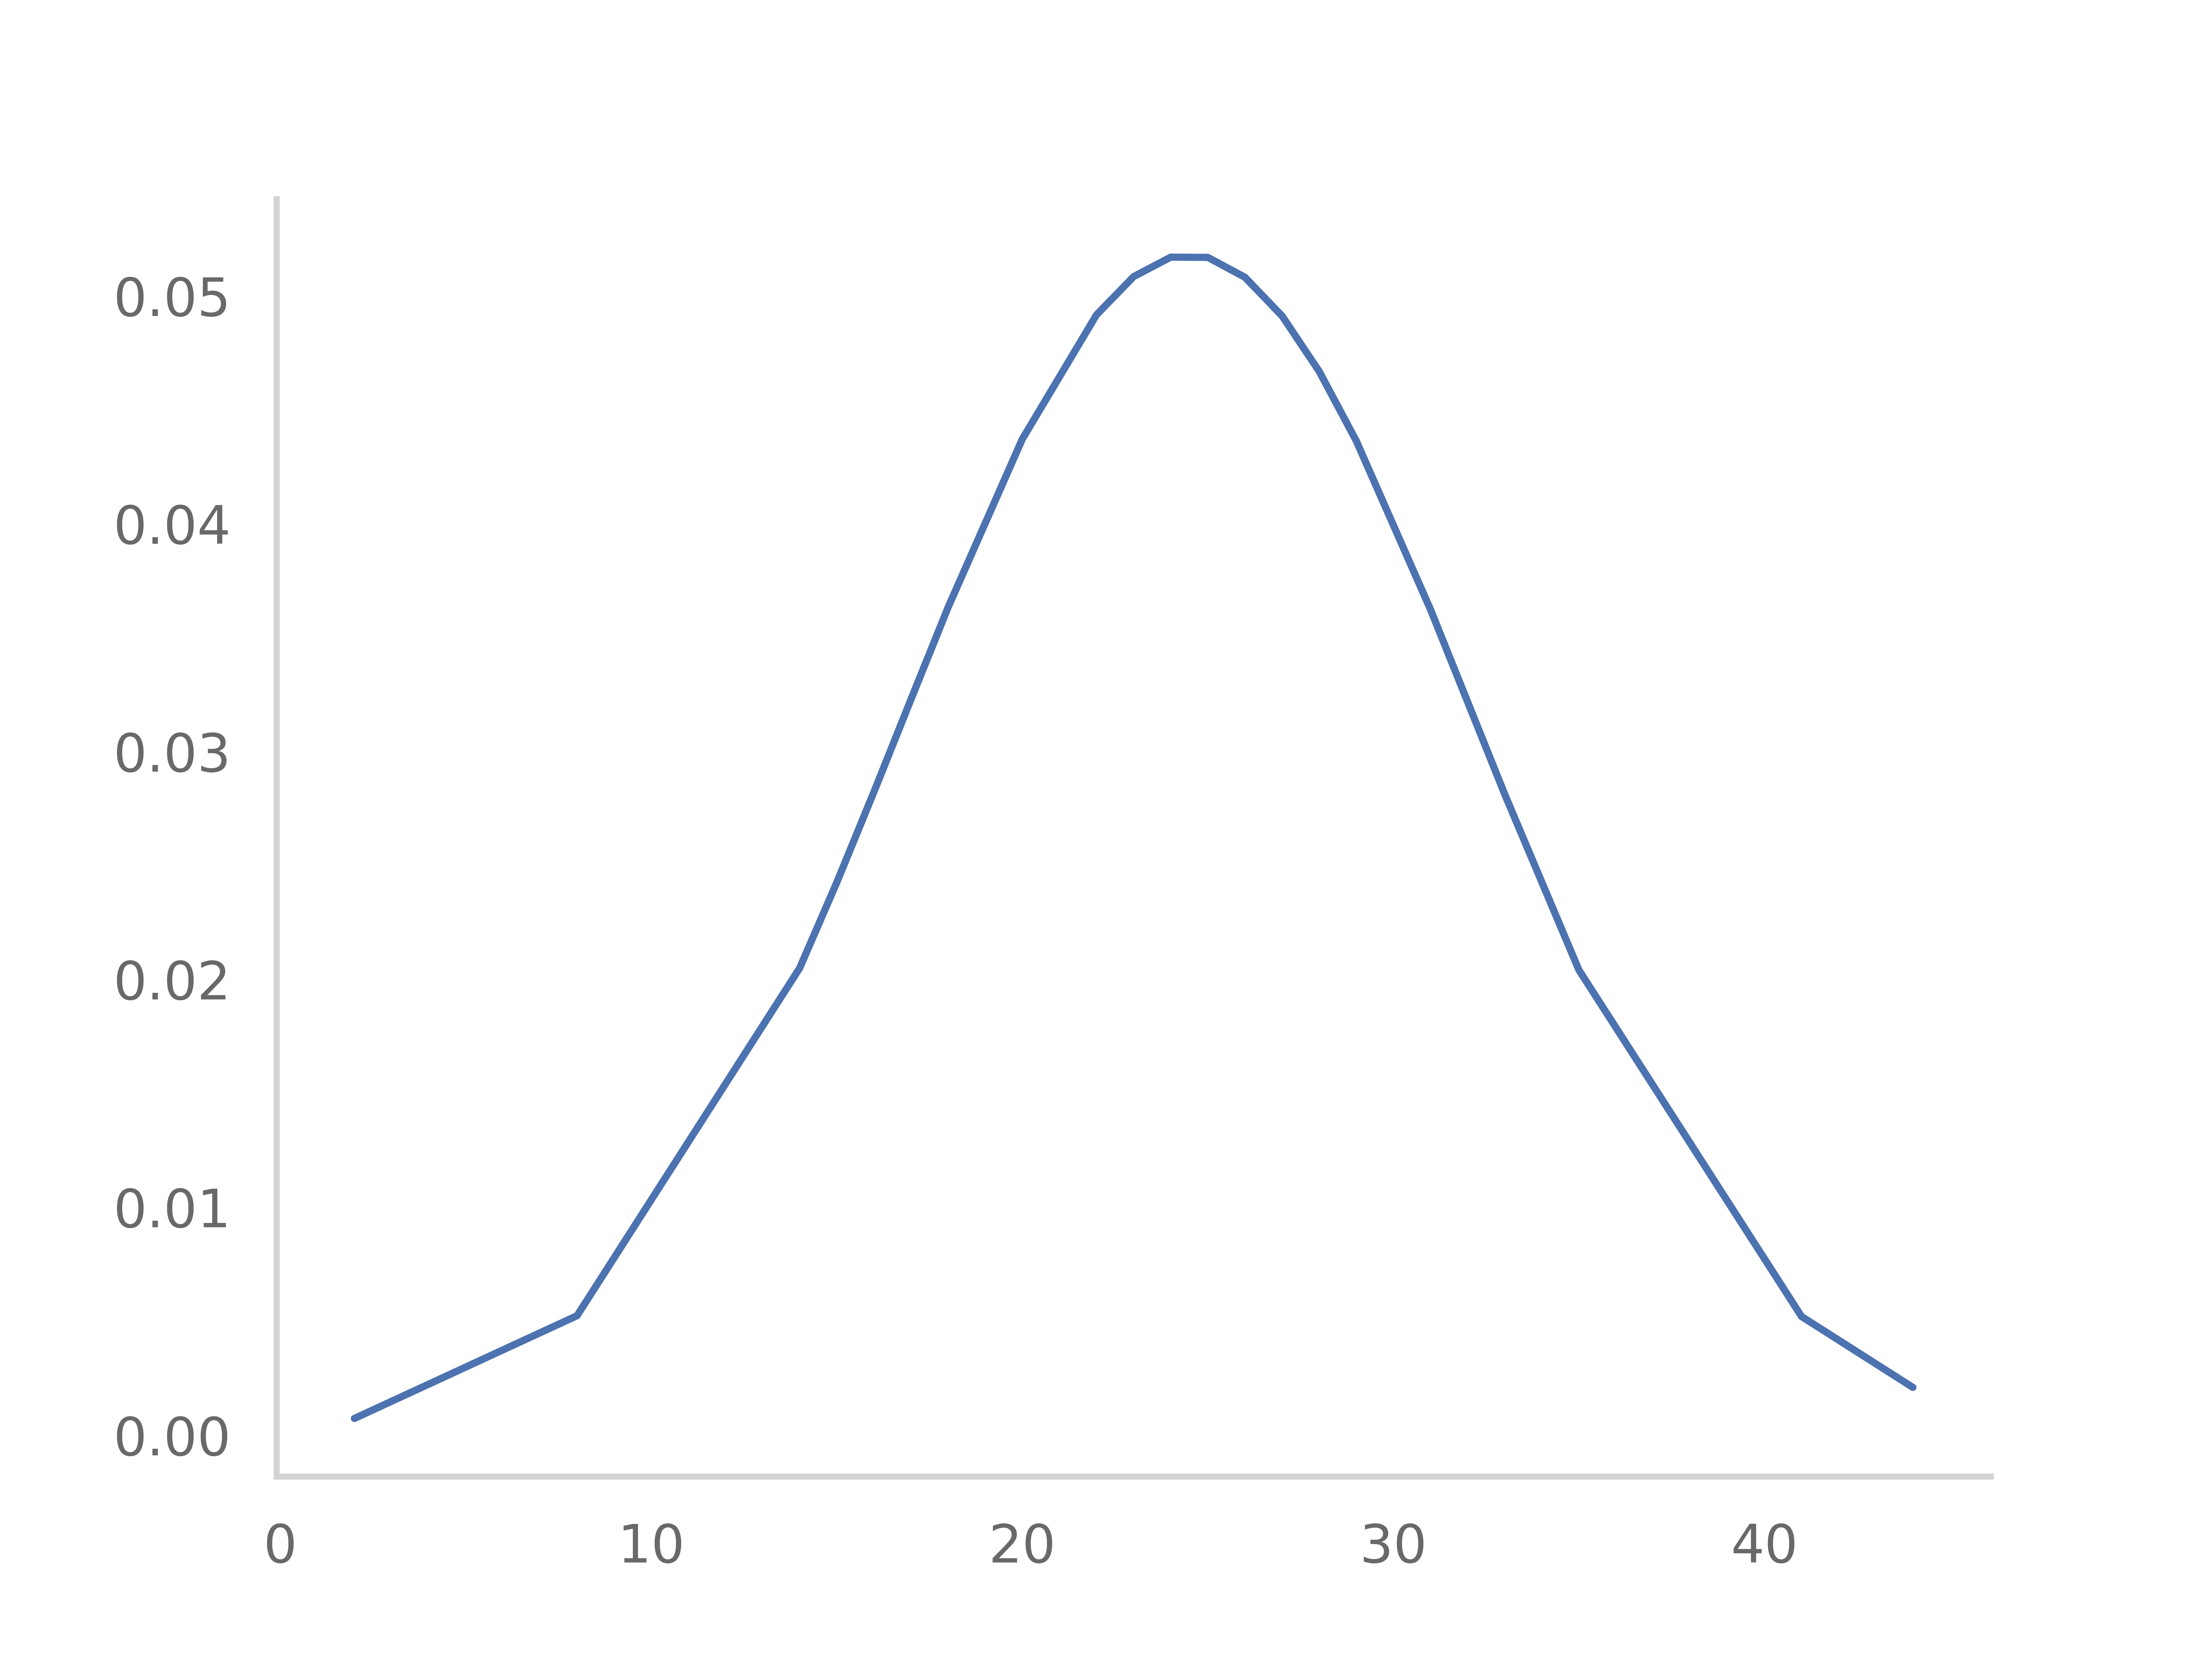
\includegraphics[width=0.75\textwidth]{species_region_invasion.png}
    \caption{Probability density function of of the number of invasions.}
    \label{fig:pdf_invasion}
\end{figure}


Due to the high sparsity of the dataset and the large computational cost, we removed from the dataset all the species that did not invade a significant amount of regions and all the regions that were not invaded by a significant number of species to reduce the space complexity of the dataset. Fig. \ref{pdf_invasion} shows how the majority of species invaded only a few number of regions. We make the assumption that a any species not invading at least 15 regions out of 276 has no relevant contribution to the model. With these restrictions the dataset has been reduced from 20473 species and 276 regions (55451 invasions in total) to 446 species and 238 regions (10275 invasions in total) number of invasions which is computationally managenable. 

\begin{figure}[H]
    \centering
    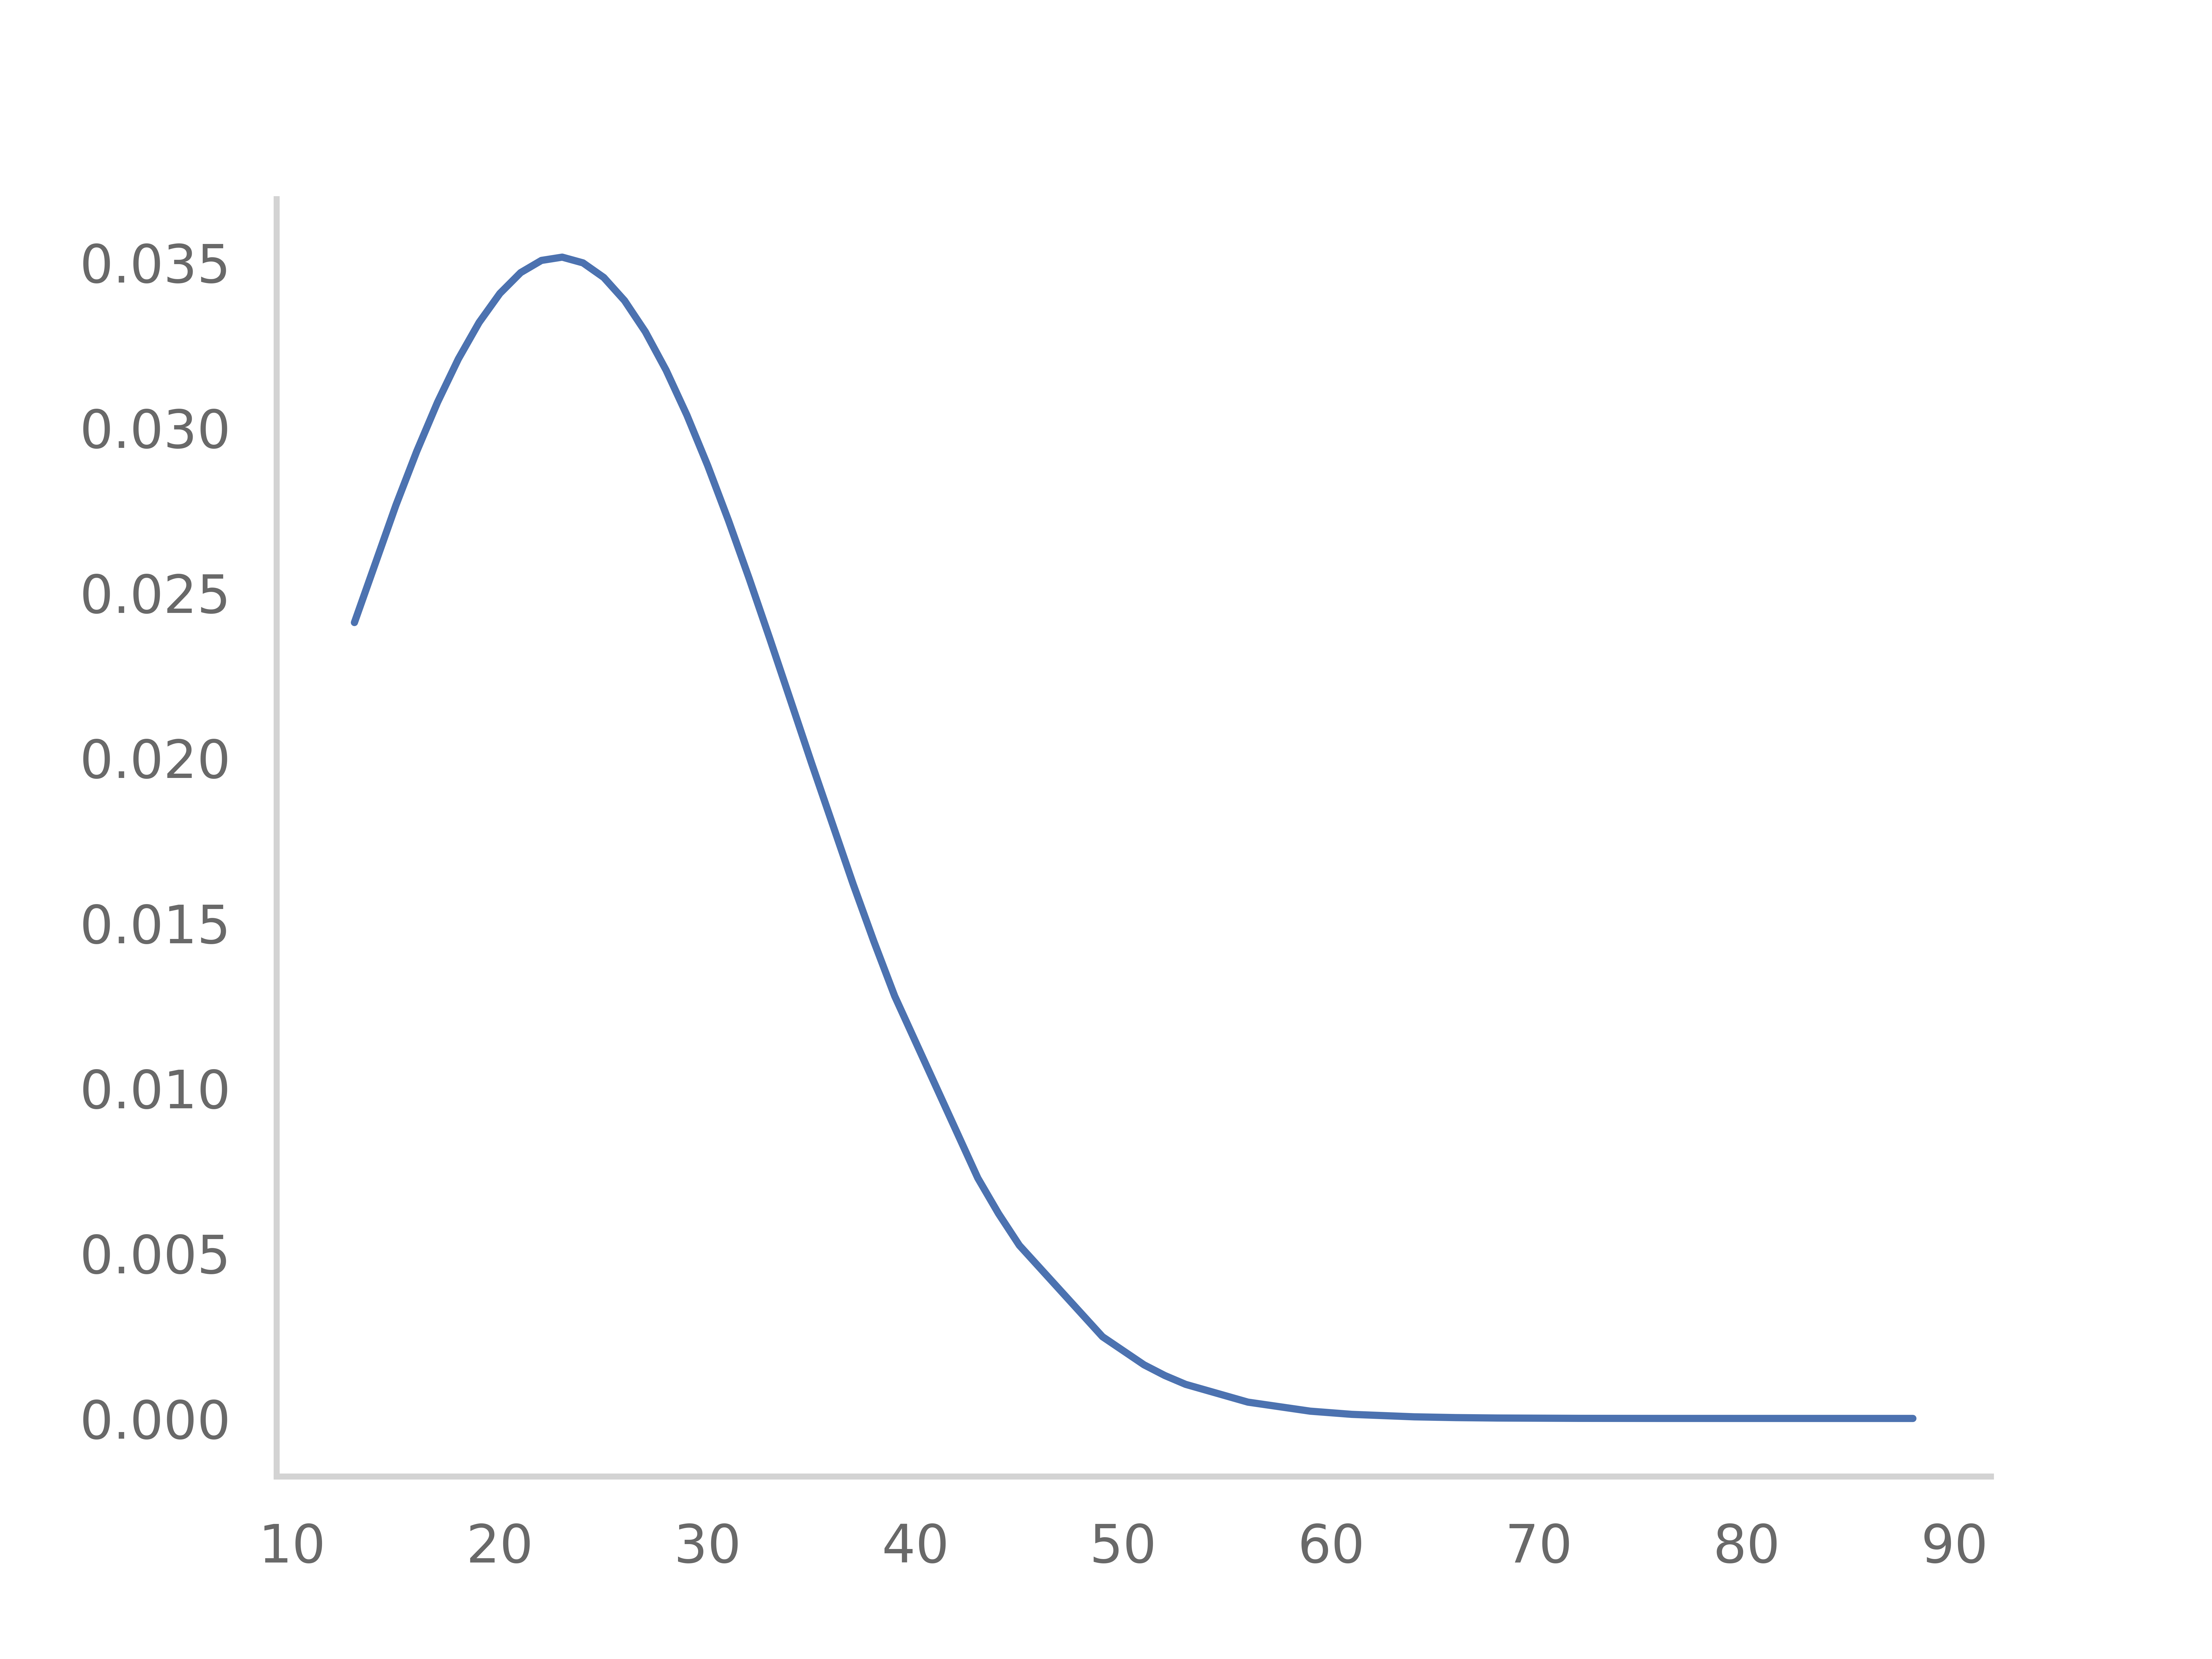
\includegraphics[width=0.75\textwidth]{species_region_invasion_filtering.png}
    \caption{Probability density function of of the number of invasions.}
    \label{fig:pdf_invasion}
\end{figure}


\subsection{Implementation specifications}
We implemented the method discussed in TODO section in Tensorflow (TODO add cite) 

%%TODO what framework do we use - how we solved the computational cost problem
The size of the dataset is problematic under a computational point of view. In particular, the inversion of the matrix TODO and the memory requirements to allocate all the dataset are large. However, due to the filtering described in the previous section and using efficient data structure by saving in memory only the non-zero entries and the indexes in a sparse matrix and by using CUDA toolokits to accelerate the computation in GPU our implementation meets the computational requirements.
 

%\section{The second, math section}
%
%\textbf{Theorem 1 (Residue Theorem).}
%Let $f$ be analytic in the region $G$ except for the isolated singularities $a_1,a_2,\ldots,a_m$. If $\gamma$ is a closed rectifiable curve in $G$ which does not pass through any of the points $a_k$ and if $\gamma\approx 0$ in $G$ then
%\[
%\frac{1}{2\pi i}\int_\gamma f = \sum_{k=1}^m n(\gamma;a_k) \text{Res}(f;a_k).
%\]
%\textbf{Theorem 2 (Maximum Modulus).}
%\emph{Let $G$ be a bounded open set in $\mathbb{C}$ and suppose that $f$ is a continuous function on $G^-$ which is analytic in $G$. Then}
%\[
%\max\{|f(z)|:z\in G^-\}=\max \{|f(z)|:z\in \partial G \}.
%\]
%
%\section[third]{A very very long section, titled ``The third section'', with
%  a rather  short text alternative (third)}
%\lipsum \texttt{Some Test}
%\lstset{language=algebra,linewidth=0.95\linewidth,breaklines=true,numbers=left,
%basicstyle=\ttfamily,numberstyle=\tiny,escapeinside={//*}{\^^M},
%mathescape=true}
%\begin{lstlisting}
%import IntSpec, ItemSpec;
%
%sort cart; //*\label{sort}
%
%constructors //*\label{begin-sig}
%create() $\longrightarrow$ cart;
%insert(cart, item) $\longrightarrow$ cart;
%observers
%amount(cart) $\longrightarrow$ int;
%transformers
%delete(cart, item) $\longrightarrow$ cart; //*\label{end-sig}
%
%axioms //*\label{begin-axioms}
%forall c: cart, i, j: item 
%
%amount(create()) $=$ 0; //*\label{begin-amount}
%amount(insert(c,i)) $=$ amount(c) $+$ price(i); //*\label{end-amount}
%delete(create(),i) $=$ create(); //*\label{begin-delete}
%delete(insert(c,i),j) $=$
%if (i =$\:$= j) c
%else insert(delete(c,j),i); //*\label{end-axioms}
%end
%\end{lstlisting}
%
%As you can easily see from the above listing \citet{bbggs:iet07}
%define something weird based on the BPEL specification
%\citep{bpelspec}.
%\nocite{*}

%\appendix %optional, use only if you have an appendix

%\chapter{Some retarded material}
%\section{It's over\dots}
%\lipsum 
%
%\backmatter
%
%\chapter{Glossary} %optional

%\bibliographystyle{alpha}
%\bibliographystyle{dcu}
\bibliographystyle{plainnat}
\bibliography{biblio}

%\cleardoublepage
%\theindex %optional, use only if you have an index, must use
	  %\makeindex in the preamble
%\lipsum

\end{document}
